\section{Geometry of $\mathbb{R}^n$}

Each vector $\begin{bmatrix}v_1\\v_2 \\ \vdots \\ v_n \end{bmatrix} \in \mathbb{R}^n$ can be visualized as an arrow going from the origin 
$(0,0, \ldots, 0)$ to the point $(v_1, v_2, \ldots, v_n)$.  In this case we'd call the \textbf{base point} the origin.

\begin{example}
$\begin{bmatrix}2\\5\end{bmatrix}$ can be visualized as the arrow between $(0,0)$ and $(2,5)$\\
  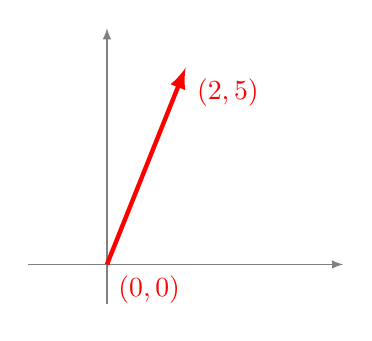
\begin{tikzpicture}[scale=.5]
    \coordinate (Origin)   at (0,0);
    \coordinate (XAxisMin) at (-2,0);
    \coordinate (XAxisMax) at (6,0);
    \coordinate (YAxisMin) at (0,-1);
    \coordinate (YAxisMax) at (0,6);
    \draw [thin, gray,-latex] (XAxisMin) -- (XAxisMax);% Draw x axis
    \draw [thin, gray,-latex] (YAxisMin) -- (YAxisMax);% Draw y axis
    \draw [ultra thick,-latex,red] (Origin) node [below right] {$(0,0)$} -- (2,5) node [below right] {$(2,5)$};
  \end{tikzpicture}
\end{example}

We can also think of any arrow from point $(a_1, a_2, \ldots, a_n)$ to point $(b_1, b_2, \ldots, b_n)$ as a vector. We've simply changed 
the \text{base point} to $(a_1, a_2, \ldots, a_n)$ instead of the origin. 

\begin{definition}
The \textbf{canonical form} of a vector from $(a_1, a_2, \ldots, a_n)$ to $(b_1, b_2, \ldots, b_n)$ is the vector 
$\begin{bmatrix}b_1-a_1 \\ b_2-a_2 \\ \vdots \\ b_n-a_n\end{bmatrix}$
\end{definition}

\begin{remark}
You can think of the canonical form of a vector is taking an arrow with the same length and direction with base point of the origin.
\end{remark}

\begin{example}
The vector from $(2,3)$ to $(3,-2)$ has canonical form $\begin{bmatrix*}[C]1\\-5\end{bmatrix*}$. Below the vector is in red and the canonical form of the vector is in blue.\\
  \begin{tikzpicture}[scale=.5]
    \coordinate (Origin)   at (0,0);
    \coordinate (XAxisMin) at (-6,0);
    \coordinate (XAxisMax) at (6,0);
    \coordinate (YAxisMin) at (0,-6);
    \coordinate (YAxisMax) at (0,6);
    \draw [thin, gray,-latex] (XAxisMin) -- (XAxisMax);% Draw x axis                                                                                                   
    \draw [thin, gray,-latex] (YAxisMin) -- (YAxisMax);% Draw y axis                                                                                                   
    \draw [ultra thick,-latex,red] (2,3) node [above right] {$(2,3)$} -- (3,-2) node [above right] {$(3,-2)$};
    \draw [ultra thick,-latex,blue] (Origin) node [above right] {$(0,0)$} -- (1,-5) node [above right] {$(3,-2)$};
  \end{tikzpicture}
\end{example}

\subsection{Scalar Multiplication and Vector Addition}

Scalar multiplication can be thought of as a  geometric operation. If $r>0$ then $r\vec{v}$ can be thought of as $v$ stretched or shrunk by real factor $r$.\\ 

\begin{tikzpicture}[scale=.5]
    \coordinate (Origin)   at (0,0);
    \coordinate (XAxisMin) at (-6,0);
    \coordinate (XAxisMax) at (6,0);
    \coordinate (YAxisMin) at (0,-6);
    \coordinate (YAxisMax) at (0,6);
    \draw [thin, gray,-latex] (XAxisMin) -- (XAxisMax);% Draw x axis                                                                                                   
    \draw [thin, gray,-latex] (YAxisMin) -- (YAxisMax);% Draw y axis                                                                                                   
    \draw [ultra thick,-latex,blue] (0,0)  -- (6,3) node[pos=0.5,above]{$r\vec{v}$};
    \draw [ultra thick,-latex,black] (Origin) -- (2,1) node[pos=0.5,above]{$\vec{v}$};;
\end{tikzpicture}

If $r<0$ then $r\vec{v}$ can be thought of as $v$ reflected through the origin then stretced or shrunk by a real factor $|r|$

\begin{tikzpicture}[scale=.5]
    \coordinate (Origin)   at (0,0);
    \coordinate (XAxisMin) at (-6,0);
    \coordinate (XAxisMax) at (6,0);
    \coordinate (YAxisMin) at (0,-6);
    \coordinate (YAxisMax) at (0,6);
    \draw [thin, gray,-latex] (XAxisMin) -- (XAxisMax);% Draw x axis                                                                                                   
    \draw [thin, gray,-latex] (YAxisMin) -- (YAxisMax);% Draw y axis                                                                                                   
    \draw [ultra thick,-latex,blue] (0,0)  -- (-6,-3) node[pos=0.5,above]{$r\vec{v}$};
    \draw [ultra thick,-latex,black] (Origin) -- (2,1) node[pos=0.5,above]{$\vec{v}$};;
\end{tikzpicture}

Vector addition can also be thought of as a geometric operation via the \textbf{parallelogram rule}. 

\begin{proposition}[The Paralelogram Rule] If $\vec{v},\vec{w} \in \mathbb{R}^n$ with then $\vec{v}+\vec{w}$ can be determined by the following:
\begin{enumerate}
\item If there is a nonzero linear combination $s\vec{v}+t\vec{w}$ equal to $\vec{0}$ then 
$\vec{v}+\vec{w}$ is either a scalar multiple of $\vec{v}$ or a scalar multiple of $\vec{w}$.

\item Otherwise $\vec{v}+\vec{w}$ is determined by the parallelogram rule:\\
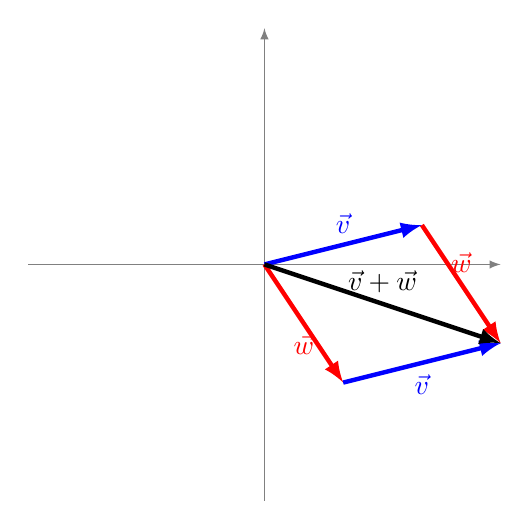
\begin{tikzpicture}[scale=.5]
    \coordinate (Origin)   at (0,0);
    \coordinate (XAxisMin) at (-6,0);
    \coordinate (XAxisMax) at (6,0);
    \coordinate (YAxisMin) at (0,-6);
    \coordinate (YAxisMax) at (0,6);
    \draw [thin, gray,-latex] (XAxisMin) -- (XAxisMax);% Draw x axis                                                                                                   
    \draw [thin, gray,-latex] (YAxisMin) -- (YAxisMax);% Draw y axis                                                                                                   
    \draw [ultra thick,-latex,blue] (0,0)  -- (4,1) node[pos=0.5,above]{$\vec{v}$};
    \draw [ultra thick,-latex,red] (4,1)  -- (6,-2) node[pos=0.5,above]{$\vec{w}$};
    \draw [ultra thick,-latex,red] (Origin) -- (2,-3) node[pos=0.5,below]{$\vec{w}$};;
    \draw [ultra thick,-latex,blue] (2,-3)  -- (6,-2) node[pos=0.5,below]{$\vec{v}$};
    \draw [ultra thick,-latex,black] (0,0)  -- (6,-2) node[pos=0.5,above]{$\vec{v}+\vec{w}$};
\end{tikzpicture}

Note that taking the base point of $\vec{w}$ to be the end point of $\vec{v}$ yeilds the same result as taking the base point of $\vec{v}$ to be the end point of 
$\vec{w}$.
\end{enumerate}
\end{proposition}
\begin{proof}
The proof of the case where there is a nonzero linear combination of $s\vec{v}+t\vec{w}=\vec{0}$ is Exercise~\ref{exercise:dependent_addition}. This case eliminates the possiblity that $\vec{v}$ and $\vec{w}$ are on the same line.

The vector $\vec{v}$ take the origin $(0,0, \ldots, 0)$ to the coordinate $(v_1, v_2, \ldots, v_n)$. 
By adding vector $w$ we take $(v_1, v_2, \ldots, v_n)$ to $(v_1+w_1, v_2+w_2, \ldots, v_n+w_n)$. 
So $v+w$ is the composite operation of taking the origin to $(v_1, v_2, \ldots, v_n)$ then to $(v_1+w_1, v_2+w_2, \ldots, v_n+w_n)$. 

Graphically we can think of this as follow the canonical form of $\vec{v}$ then base $w$ at the endpoint of $v$ to get $\vec{v}+\vec{w}$. Since we can do the same thing starting with $w$, this makes a parallelogram as long as $\vec{v}$ and $\vec{w}$ are not on the same line.
\end{proof}

\begin{example} 
Let $\vec{v}=\begin{bmatrix} 1 \\ 3 \end{bmatrix}$ and $\vec{w}=\begin{bmatrix*}[C] -5 \\ 2 \end{bmatrix*}$. We can identify all vectors in $\mathbb{R}^n$ as a linear combination of these two geometrically. Since the canonical forms of$\vec{v}$ and $\vec{w}$ are not in the same line in $\mathbb{R}^n$, $\vec{v}+\vec{w}$ forms a parallelogram. Below we mark all the integer linear combination endpoints of $m\vec{v}+n\vec{w}$ where $n$ and $m$ are integers. This makes a shape called a lattice:
\begin{center}
\includegraphics[scale=.5]{Rn/vw_graph1.pdf}
\end{center}

We can see below that the vector $\begin{bmatrix*}[C]9 \\ -7 \end{bmatrix*}$ can be written by the linear combination $(-1)\vec{v}+(-2)\vec{w}$. It doesn't even mater what path we use to get there since we can use the associative properties of vector addition and the distributive property of vector addition and scalar multiplication.
\begin{center}
\includegraphics[scale=.5]{Rn/vw_9n7_graph1.pdf}
\end{center}

It's not a very large stretch to include vectors with endpoints on the rest of the plane since all we need to allow is any real linear combination $r\vec{v}+t\vec{w}$ where $r$ and $t$ are real numbers. For instance we can add in the endpoint $(3,3)$ by taking $\frac{21}{17}\vec{v}+\frac{-6}{17}\vec{w}$\\
\begin{center}
\includegraphics[scale=.5]{Rn/vw_graph2.pdf}\
\end{center}
\end{example}

\subsection{Linear Dependence and Linear Independence}

\subsection{Some Geometric Linear Transformations}

\subsection{Dot Product, Distance and Angle between vectors}

